\subsection{Проектування моделей даних}
\label{subsec:data-models}

Добре розроблена модель даних є основою для точного представлення і маніпулювання транспортною мережею та пов'язаними з нею об'єктами. Основна мета моделі даних - зафіксувати основні елементи, такі як зупинки, маршрути, розклади та їх взаємозв'язки, забезпечуючи комплексне представлення транспортної системи. Це дозволяє ефективно зберігати, знаходити та маніпулювати даними, що дає нам змогу виконувати різні аналізи та операції з пошуку маршрутів.

Під час процесу моделювання даних ретельна увага приділяється відповідним структурам даних і взаємозв'язкам для точного відображення реальної транспортної мережі. Це передбачає визначення таких об'єктів, як вузли (що представляють зупинки або місця), ребра (що представляють сполучення між зупинками) та атрибути, які описують різні властивості цих об'єктів.

Для представлення моделі даних ми використовуємо поєднання концепцій реляційних баз даних та графових структур даних. Реляційні бази даних забезпечують структурований підхід для зберігання та запитів до великих обсягів даних, в той час як графи пропонують інтуїтивно зрозуміле представлення зв'язків між об'єктами, що робить їх ідеальними для сценаріїв планування маршрутів.

Використовуючи можливості моделі даних, пристосованої до конкретних потреб, можна ефективно вирішувати завдання зберігання, пошуку та маніпулювання даними. Це закладає основу для наступних етапів проекту, включаючи реалізацію алгоритмів та оптимізацію маршрутів.

Модель "Station" слугує фундаментальною сутністю для представлення окремих зупинок або місць у транспортній мережі. Вона містить основну інформацію, таку як назва або ідентифікатор станції, географічні координати, що визначають її точне місцезнаходження,  створюючи чітку структуру категоризації.

Модель "Route" відіграє центральну роль у визначенні конкретних маршрутів або ліній у транспортній системі. Вона інкапсулює такі важливі атрибути, як назва або ідентифікатор маршруту. Крім того, модель "Route" встановлює зв'язок "багато-до-багатьох" з моделлю "Station", що дозволяє нам точно представити послідовність зупинок на маршруті.

Для відображення з'єднань або зв'язків між "Station" та "Route" ми використовуємо модель "Connection". Ця модель включає такі поля, як станція відправлення та станція призначення, що представляють початкову та кінцеву точки з'єднання відповідно. Вона також включає такі атрибути, як розклад відправлень.

Для відображення проміжків, з яких складається "Connection" розроблена модель "Waypoint". Вона представляє відрізок між зупинками(на станціях представлених моделлю "Station"). Ця модель дозволяє відображати проміжні точки або зупинки на маршруті, що сприяє точному моделюванню та ефективній обробці даних. Підтримуючи зв'язок з моделями "Station" та "Route", модель "Waypoint" фіксує пов'язану станцію для кожної точки маршруту і забезпечує збереження порядку або послідовності точок на маршруті.

\begin{figure}[!h]
    \centering
    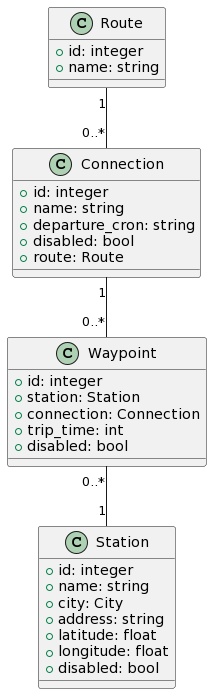
\includegraphics[scale=0.6]{content/chapters/2-implementation-methods/assets/img/models_diagram.png}
    \caption{Діаграма описаних моделей}
    \label{fig:bfs}
\end{figure}


Включаючи ці ретельно розроблені моделі в наш проект, ми створюємо надійну і структуровану структуру представлення даних. Ця основа дозволяє нам ефективно працювати з різноманітними типами транспорту та конфігураціями маршрутів. Модель Station забезпечує детальне представлення окремих зупинок, модель Route відображає загальну структуру маршрутів, модель Connection встановлює зв'язки між станціями, а модель Waypoint враховує складні конфігурації маршрутів. Разом ці моделі забезпечують ефективне зберігання, пошук та маніпулювання даними транспортної системи, сприяючи точному та оптимізованому плануванню маршрутів.